\section{Numerical Results}

  With a defined method and computational setup a varaity of simulations can be run to observe the accuracy and behaviour of the method.
  An examination a typical simulation will show if the expected behaviour is observed, validating the method as functioning.
  A convergence analysis for the method can be done to confirm that solutions from different grid sizes approche a single solution as they become more precise.
  This convergence test will also show the thresholds for an accurate simulation result, to help reduce the computiation times.
  With a well-established method, the comparison between semi- and fully-implicit methods can be done.

\subsection{Basic Simulations}

  Using Algorithm \ref{alg:iterateCM}, simple scenarios can be tested as a first verification on the method.

  % Too simple/useless visual. Instead maybe have a graph of the standard deviation between gridpoints and show that it stays 0 (or constant?) with time.
  %
  %The most simple test would be homogenous initial conditions, $M = 0.1, C = 1 \forall x \in \Omega$.
  %This test would serve mainly as a confirmation that the method can solve (\ref{equ:model_system}) with the most trivial of initial conditions accurately.
  %The solutions in Figure \ref{fig:basic_homo} show that with homogenous initial conditions, the solution remains homogenous with time.
  %
  %\begin{figure}
  %  \centering
  %  \begin{tabular}{c}
  %  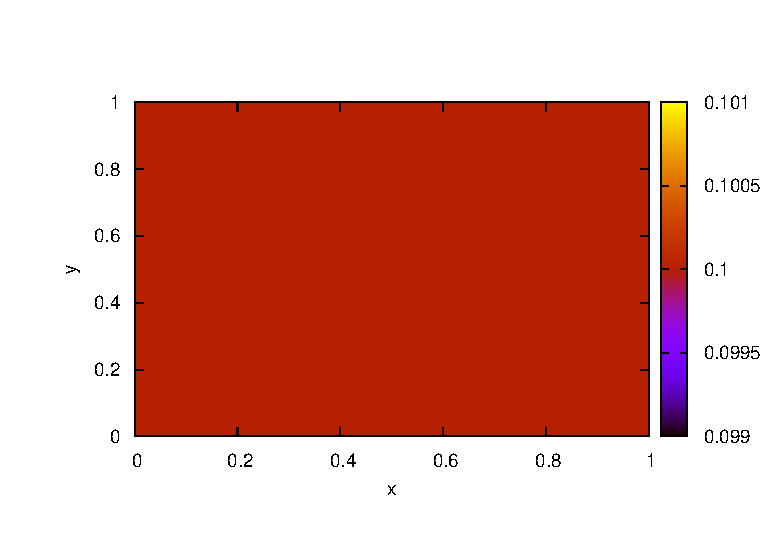
\includegraphics[scale = 0.8]{basic_homo_t0} \\ 
  %  (a) \\
  %  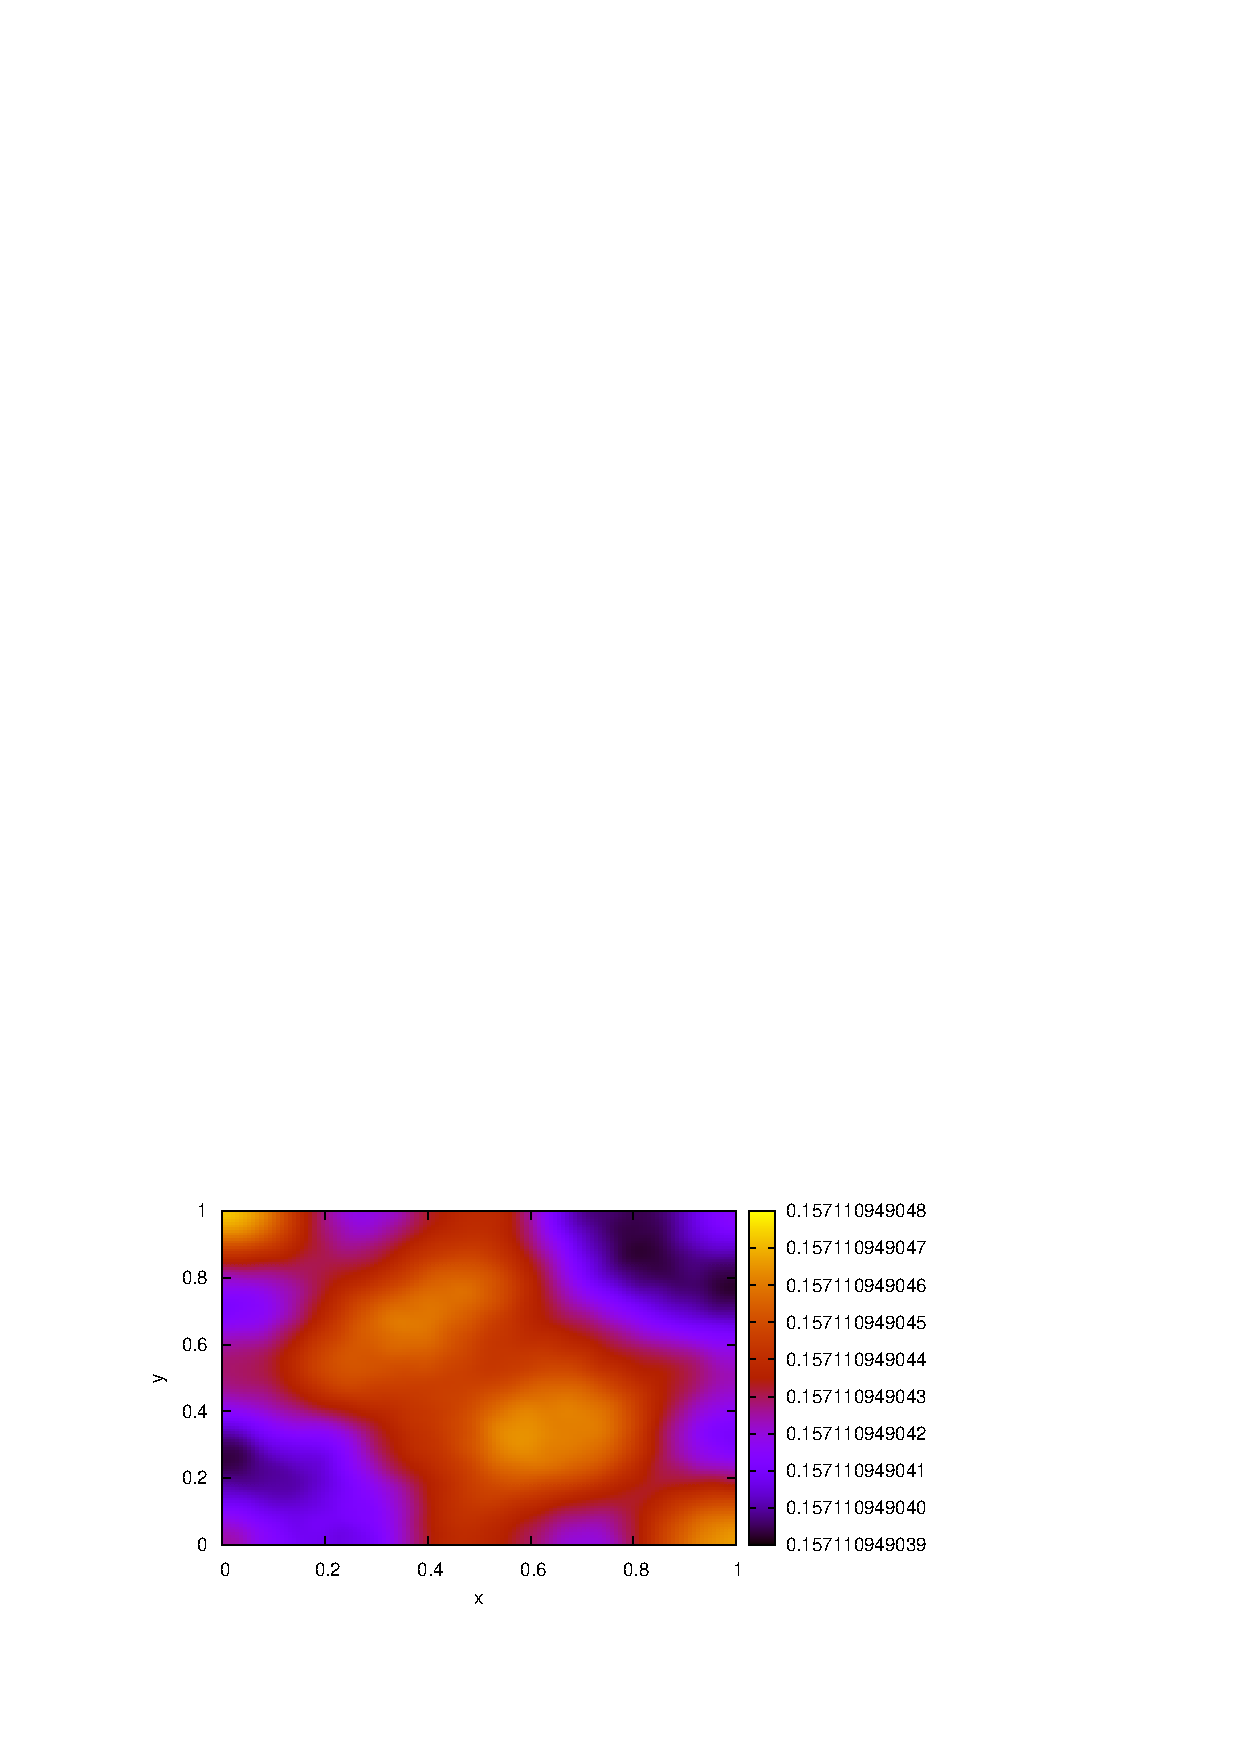
\includegraphics[scale = 0.8]{basic_homo_t10} \\
  %  (b)
  %  \end{tabular}
  %  \caption{Basic homogenous solutions, with $M = 0.1, C = 1 \forall x \in \Omega$. 
  %    The solution stay homogenous with time, as seen by comparing (a) the initial solution at $t = 0$, and (b) at $t = 10$.}
  %  \label{fig:basic_homo}
  %\end{figure}
  

  %!% These show that the spatial discretization didn't introduce andy sink/sources of biomass.
  %!% add to this the spherica IC, one that hits the boundaries but only show the output that doesn't hit boundary
  A simple test would test if the diffusion reaction model works for the propagation of the biomass.
  Having, all of the biomass on one boundary of $\Omega$ would show the spatial diffusion across the region.
  With the initial conditions,
  \begin{equation} \label{equ:basic_init_trav_wave}
    \begin{aligned}
    M &= \begin{cases}
      -\left( \frac{h}{d^4} \right) x^4 + h & \text{if } y \le d \\
      0 & \text{otherwise}
    \end{cases} \\
    C &= 1
    \end{aligned}
  \end{equation}
  where $h = 0.1$ and $d = \frac{5}{128}$.
  Here, $h$ and $d$ represent the height and depth of the innoculation site. 
  The solution in Figure \ref{fig:basic_trav} show that, with initial conditions given in (\ref{equ:basic_init_trav_wave}), the solution propagate consistently with time.
  
  \begin{figure}
    \centering
    \begin{tabular}{c}
      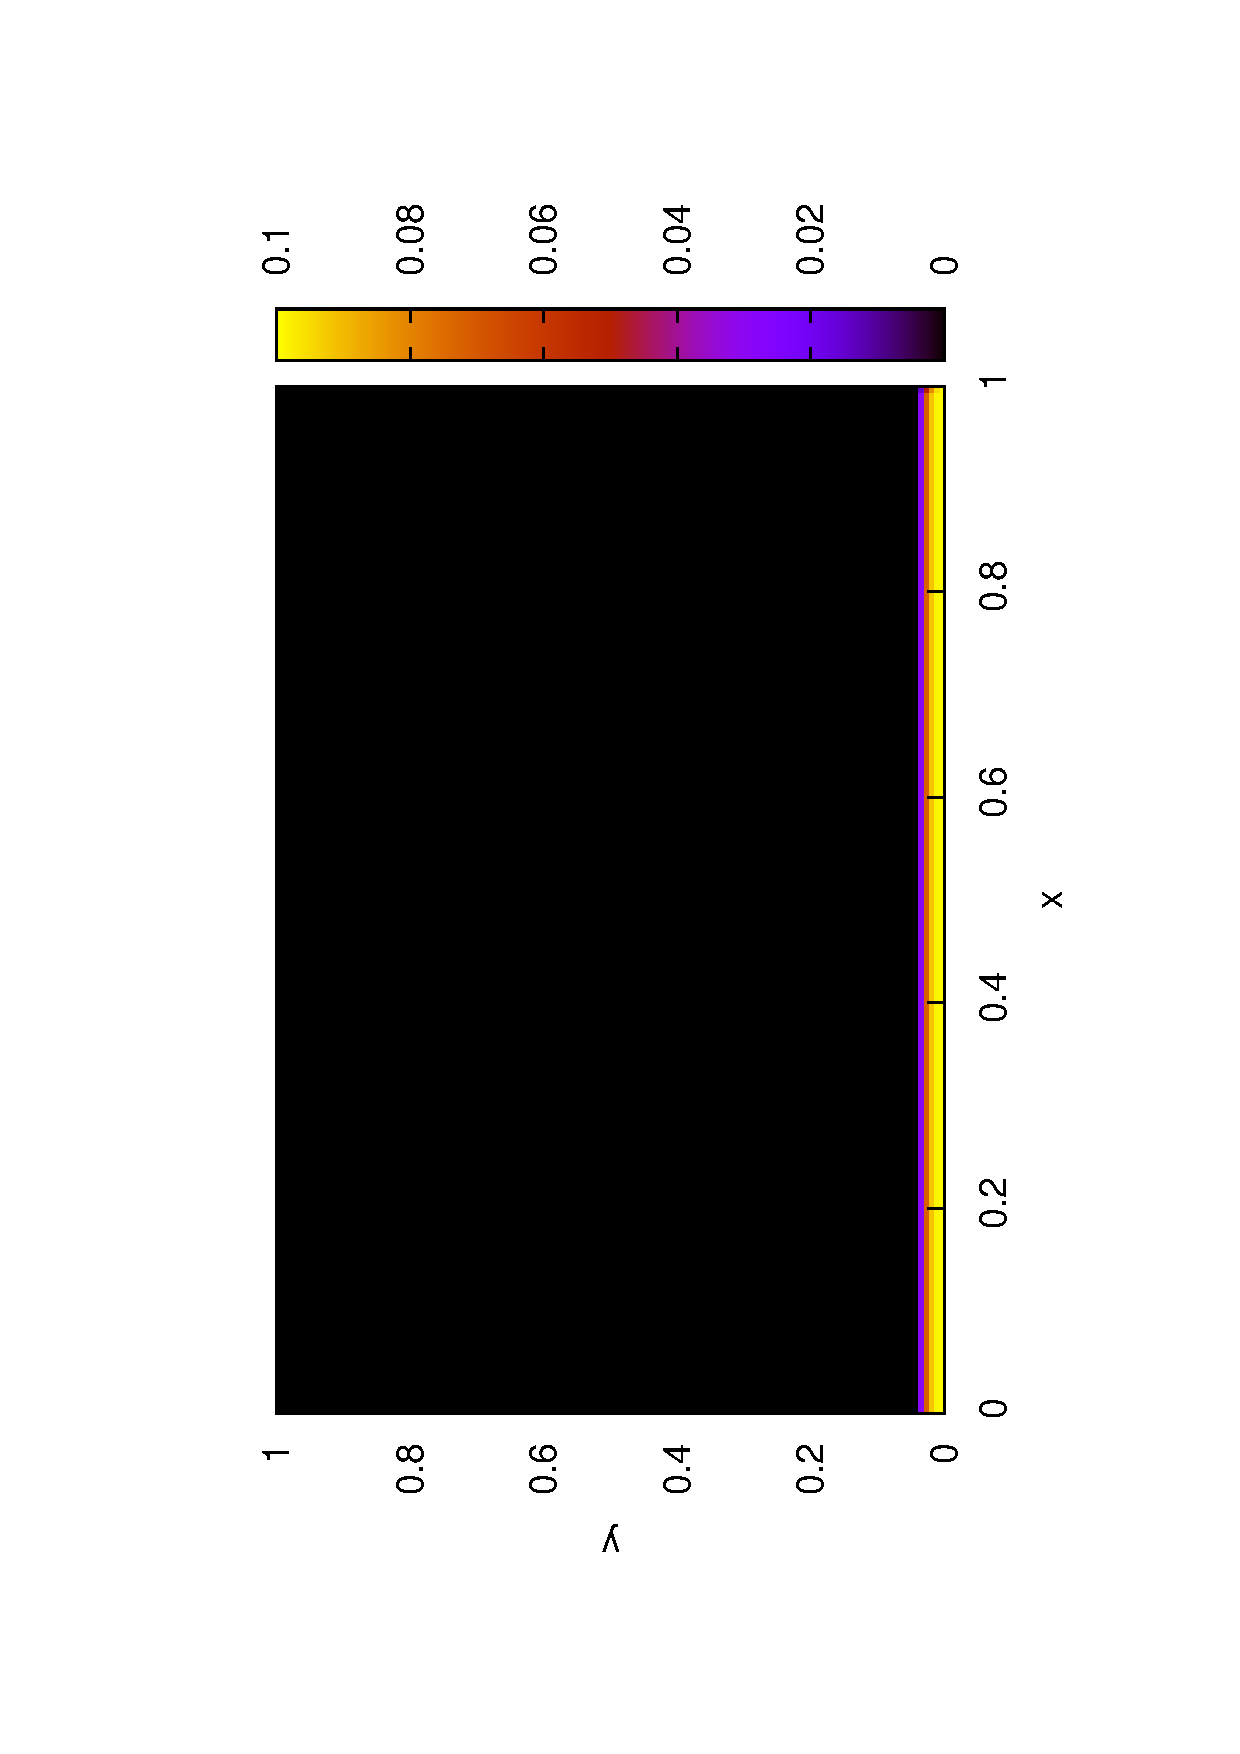
\includegraphics[scale = 0.5, angle = 270]{basic_trav_t0} \\
      (a) \\
      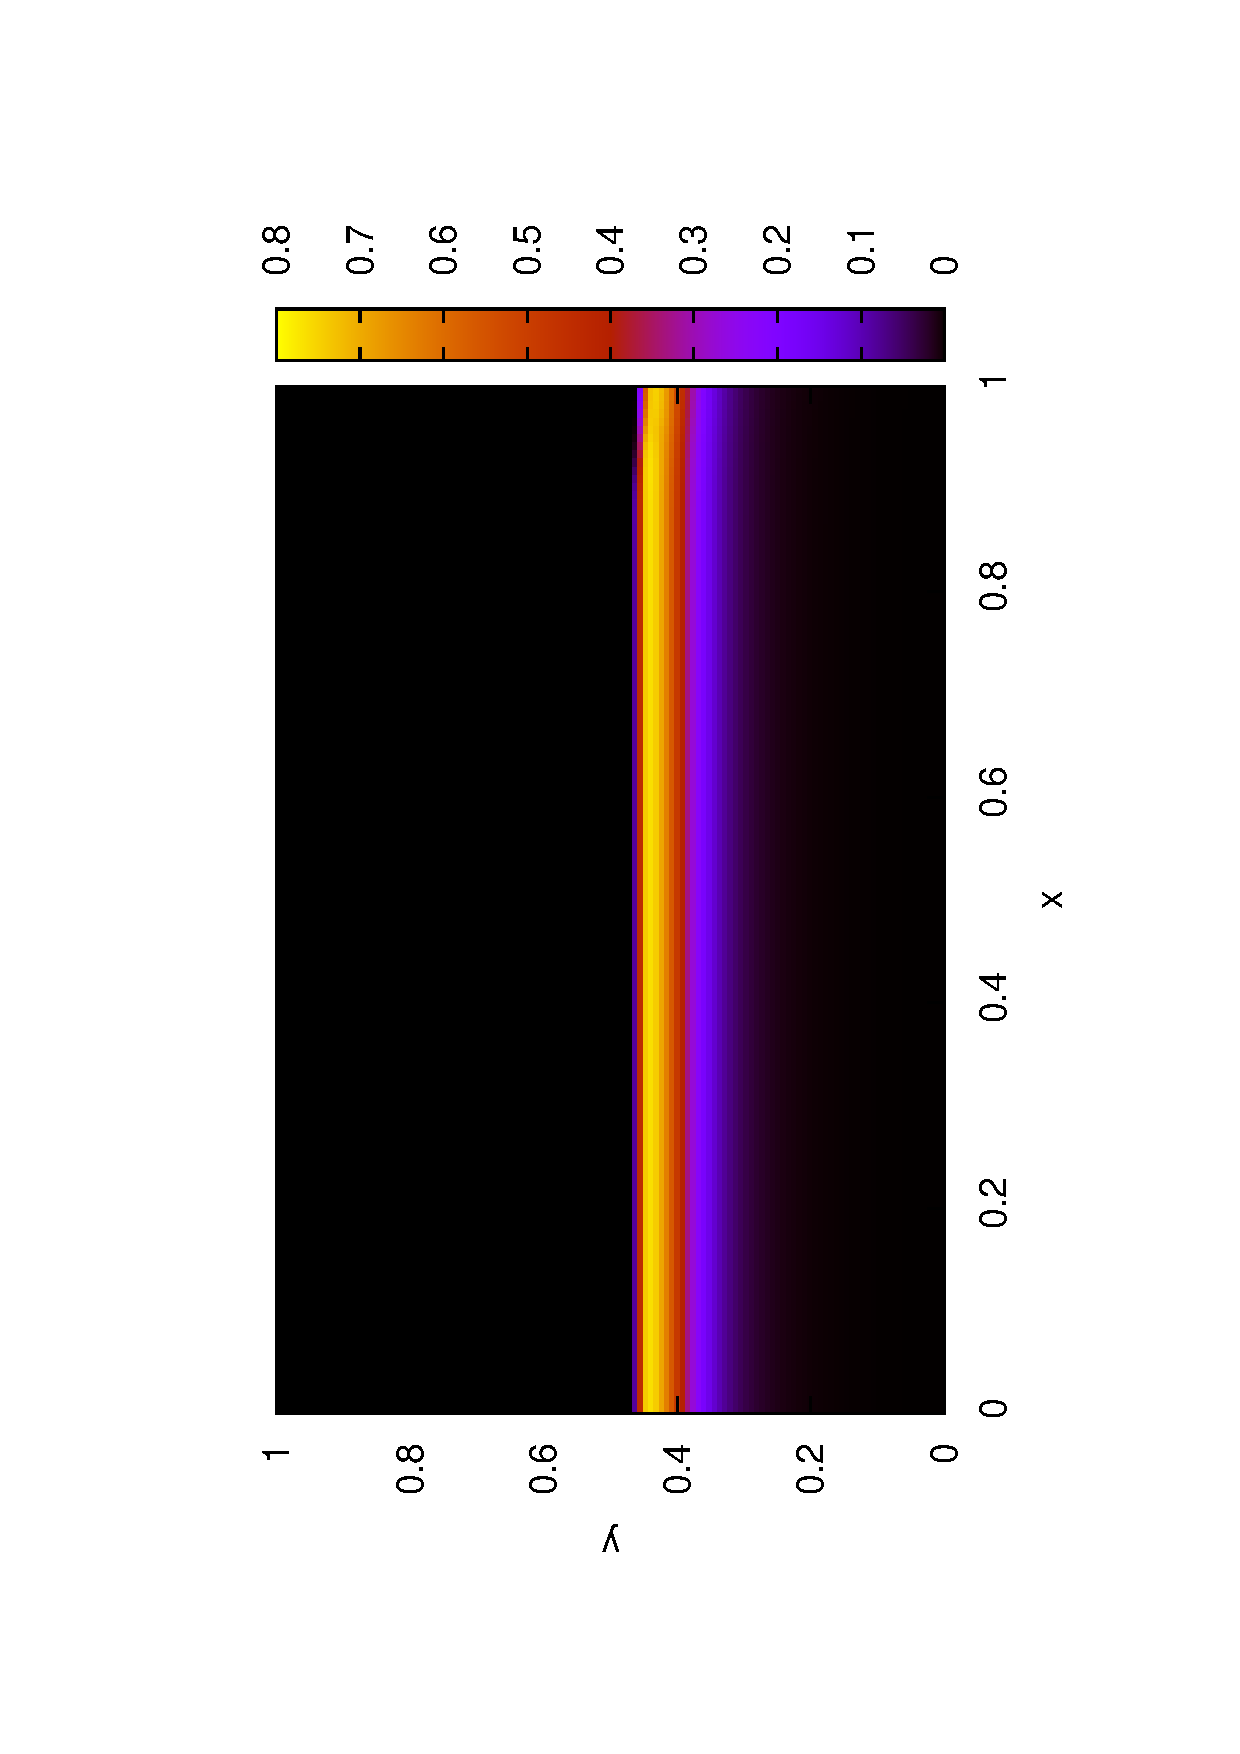
\includegraphics[scale = 0.5, angle = 270]{basic_trav_t40}\\
      (b) 
    \end{tabular}
    %!% Maybe in here try having a 2x2 grid; (M, C) as columns, and (t = 0, t = 40) as rows
    \caption{Solutions for $M$ with initial conditions given in (\ref{equ:basic_init_trav_wave}) at (a) $t = 0$ and (b) $t = 40$.}
    \label{fig:basic_trav}
  \end{figure}

  %!% Mention here that the testcase is the spherical IC.
  %!% Show what happens when it hits the boundary (should mess with total biomass a bit)
  %!% If its bad enough, show that making the grid more refined reduces this (or time step maybe?)
  %!% This shows that the newmann BC doesn't destroy mass (or produce)
  The total amount of biomass has no known exact value, given the choice of growth rate function.
  However, the amount of total biomass can be predicted to grow exponentially if the growth rate function, $F(C)$ from (\ref{equ:model_functions}), was replaced with a constant.
  This can be checked by tracking the total biomass, called $T_{M}(t)$, with the changed growth rate function:
  \begin{equation} \label{equ:F_constant}
    F(C) = a
  \end{equation}
  Tracking $T_{M}(t)$ can be done by,
  \begin{equation} \label{equ:total_biomass}
    T_{M}(t) = \int_{\Omega} M(t) dx.
  \end{equation}
  Numerically, this is computed by  grid-wise summation,
  \begin{equation}
    T_{M}(t^k) \approx T_{M}^{k} = \frac{ \sum^n_i \sum^m_j M^{k}_{i,j} }{nm}
  \end{equation}
  %!% Why is this next line have \frac{1}{3812}... should maybe show the calculations that made that values'; i.e. solve y = y0*\exp^{k}
  Figure \ref{fig:basic_growth} shows that the total biomass is as expected, since it matchs the curve of $\frac{1}{3812.5}*e^{k}$, an exponential function.

  \begin{figure}
    \centering
    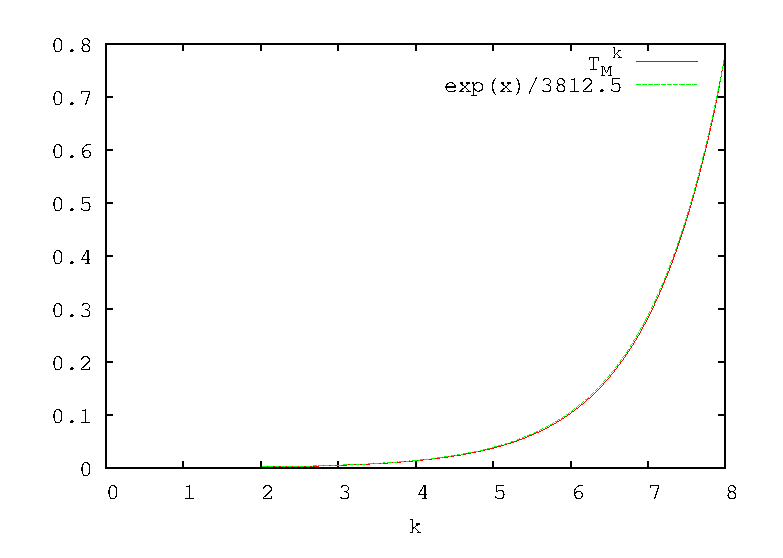
\includegraphics[scale = 0.9]{basic_growth}
    \caption{Plot of total biomass, $T_{M}^{k}$, for $k = 0,1,...,20$.}
    \label{fig:basic_growth}
  \end{figure}
  
  %!% add mass -conseration between M and C by checking that $M' + \gamma C' = 0$; ie total mass is constant
  %!% Show here the pre-work of integrating over the domain and that the spatial term dissapers and all thats left is the growth terms in both M and C.
  %!% If its interesting, show a graph of M'+gama C vs. t, and try to explain/justify the changes it makes (unless its 0, then just report that its zero and say DATA NOT SHOWN.

\subsection{Convergence Analysis}
  %!%To validate the accuracy of the method, convergence analyses on the spatial and temporal discretizations will need to be made. 
  To validate the accuracy of the method, convergence analyses on the spatial discretizations will need to be made. 
  Then the comparison between the semi- and fully-implicit method established in Algorithm \ref{alg:iterateCM} can investigated.
  First, a metric must be formed to enable consistent comparisons between different simulation solutions. 
  This metric will be referred to as the error. %!% Find a better name fore the norm...

\subsubsection{Error Computations}

  The error is computed by taking the relative normed-difference between two solution in the following fashion:
  \begin{equation} \label{equ:error_comp}
    %!% Maybe at some point try \frac{||u_1 - u_2||}{||u_1|| + ||u_2||}
    \epsilon_{sol} = \frac{||u_1 - u_2||}{||u_2||}
  \end{equation}
  where $u_1$ represents one simulation solution and $u_2$ represents the solution that is theoretically more accurate.
  The theoretical accuracy of $u_2$ derives from the fact that most comparisons will be done between solutions that vary in only $\Delta x$ or between semi- and fully- implicit.
  These are understood to have the relation that a smaller $\Delta x$, and that the fully-implicit method is to be more accurate.
  There is an assumption that both $u_1$ and $u_2$ have the same number of grid points, so that the difference can be taken grid-wise.
%!%The theoretical accuracy of $u_2$ derives from the fact that most comparisons will be done between solutions that vary in only $\Delta x$, $\Delta t$, or between semi- and fully- implicit.
%!%  These are understood to have the relation that a smaller $\Delta x$ and $\Delta t$ will be more accurate, and that the fully-implicit method is to be more accurate.


  The results of the error computations, named $\epsilon_{sol}$, is a numerical value for the difference between two solutions.
  This depends on the normed used during the computations.
  Here three norms will be used:
  \begin{equation}  \label{equ:norm_l1}
    \ell_1: ||u||_1 = \sum_{\pi(i,j)}^{nm} |u_{i,j}|
  \end{equation}
  \begin{equation}  \label{equ:norm_l2}
    \ell_2: ||u||_2 = \sqrt{\sum_{\pi(i,j)}^{nm} (u_{i,j})^2}
  \end{equation}
  \begin{equation}  \label{equ:norm_linf}
    \ell_\infty: ||u||_\infty = \max_{\substack{i=1,\ldots,n \\j=1,\ldots,m}} |u_{i,j}|
  \end{equation}
  These different norms will all be used to create a broader understanding of the error.
  This creates three distinct values for $\epsilon_{sol}$, named $\epsilon_{\ell_1}$, $\epsilon_{\ell_2}$, and $\epsilon_{\ell_\infty}$; each named for the norm used during the computation.
  
 %!% \item What program did I use? (R probably....)
 %!% \item Maybe run though a trivial Fisher equation problem to confirm that it works ?
  % Also mention the Accuracy of the solutions by using the norm of each solution compared to the  most accurate one.... (Maybe take a solution at a higher grid resolution?, not sure what to do here)

\subsubsection{Grid Size Convergence}
%!% Just show the results and state it is slow to converge when F(C) is dependent on C (double check with the older versions of code)
  To observe the validity of the method, a test on the convergence of solutions based on the spatial discritization is done.
  This will involve using the same simulation described in (\ref{equ:basic_init_trav_wave}) due to the simplicity. 
  The convergence will be tracked with all three forms of $\epsilon_{sol}$
%!% Fix flow of this section
  Since there exist a difference in the number of grid points between the different solutions, $u_1$ and $u_2$, only the grid points in the more coarse refinement will be used.
  This places a limitation on the selection of grid-sizes and so they will follow the series $s(n) = 2^{n-1}+1$ for $n \in \mathbb{Z}$.
  So that the grid points can line up, without any use of linear interpolation, grid refine must be using $s(n)$ instead of the typical grid doubling of $2^{n}$. 
  This is illustrated in Figure \ref{fig:grid_point_lineup}.


  \begin{figure}
    \centering
    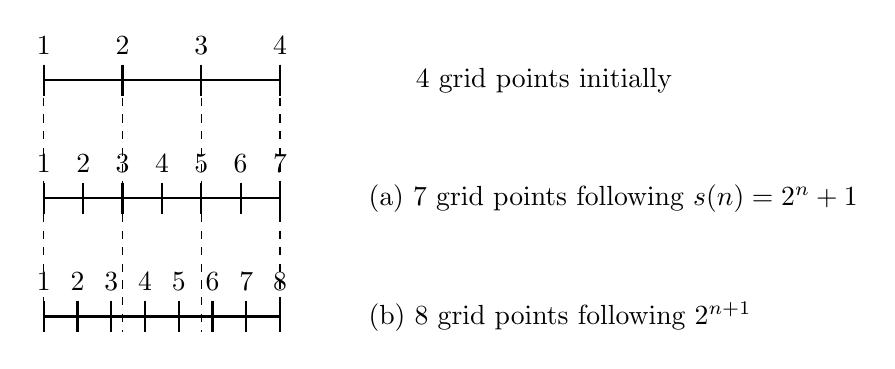
\begin{tikzpicture}
      \draw [dashed] (0, 4.2) -- (0, 0.8);
      \draw [dashed] (1, 4.2) -- (1, 0.8);
      \draw [dashed] (2, 4.2) -- (2, 0.8);
      \draw [dashed] (3, 4.2) -- (3, 0.8);
  
      \draw [thick] (0,4) -- (3,4);
      \draw [thick] (0, 4.2) -- (0, 3.8);
      \draw [thick] (1, 4.2) -- (1, 3.8);
      \draw [thick] (2, 4.2) -- (2, 3.8);
      \draw [thick] (3, 4.2) -- (3, 3.8);
  
      \node [right] at (4.6, 4) {4 grid points initially};
      \node [above] at (0,4.2) {1};
      \node [above] at (1,4.2) {2};
      \node [above] at (2,4.2) {3};
      \node [above] at (3,4.2) {4};
  
      \draw [thick] (0, 2.5) -- (3, 2.5);
      \draw [thick] (0, 2.7) -- (0, 2.3);
      \draw [thick] (0.5, 2.7) -- (0.5, 2.3);
      \draw [thick] (1, 2.7) -- (1, 2.3);
      \draw [thick] (1.5, 2.7) -- (1.5, 2.3);
      \draw [thick] (2, 2.7) -- (2, 2.3);
      \draw [thick] (2.5, 2.7) -- (2.5, 2.3);
      \draw [thick] (3, 2.7) -- (3, 2.3);
  
      \node [right] at (4, 2.5) {(a) 7 grid points following $s(n)=2^n +1$};
      \node [above] at (0, 2.7) {1};
      \node [above] at (0.5, 2.7) {2};
      \node [above] at (1, 2.7) {3};
      \node [above] at (1.5, 2.7) {4};
      \node [above] at (2, 2.7) {5};
      \node [above] at (2.5, 2.7) {6};
      \node [above] at (3, 2.7) {7};
  
      \draw [thick] (0, 1) -- (3, 1);
      \draw [thick] (0.000, 1.2) -- (0.000, 0.8);
      \draw [thick] (0.429, 1.2) -- (0.429, 0.8);
      \draw [thick] (0.857, 1.2) -- (0.857, 0.8);
      \draw [thick] (1.286, 1.2) -- (1.286, 0.8);
      \draw [thick] (1.714, 1.2) -- (1.714, 0.8);
      \draw [thick] (2.143, 1.2) -- (2.143, 0.8);
      \draw [thick] (2.571, 1.2) -- (2.571, 0.8);
      \draw [thick] (3.000, 1.2) -- (3.000, 0.8);
  
      \node [right] at (4, 1) {(b) 8 grid points following $2^{n+1}$};
      \node [above] at (0.000, 1.2) {1};
      \node [above] at (0.429, 1.2) {2};
      \node [above] at (0.857, 1.2) {3};
      \node [above] at (1.286, 1.2) {4};
      \node [above] at (1.714, 1.2) {5};
      \node [above] at (2.143, 1.2) {6};
      \node [above] at (2.571, 1.2) {7};
      \node [above] at (3.000, 1.2) {8};

      %!% Maybe try doing a 2D explaination. Showing the grids in an isometric plane in a - b - c format on one row. Then have horizontal dashed lines showing the matching (and not matching) grid-points ??
  
    \end{tikzpicture}
    \caption{Visualization in 1D explaining the use of $s(n) = 2^{n} + 1$ instead of $2^{n+1}$ to control the grid size selection. 
      When the number of grid points are (b) doubled they do not lineup with the grid points of the previous discritization.
      With (a) this problem does not exist.}
    \label{fig:grid_point_lineup}
  \end{figure}

  
  %!% Makes this use log graph and maybe its a stragith line.
  %!% Also have graphs of how the quatilites of interest change with grid-size (and with t?)
  %!% Maybe have a 2D plot of x = \delta x, y = \delta t, z = \epsilon. showing how it (should) decrease with \delta x and \t.
      %!% to the above graph, can later add computation time to it to justify the choice in \delta t and \delta x for the later simulations
  \begin{figure}
    \centering
    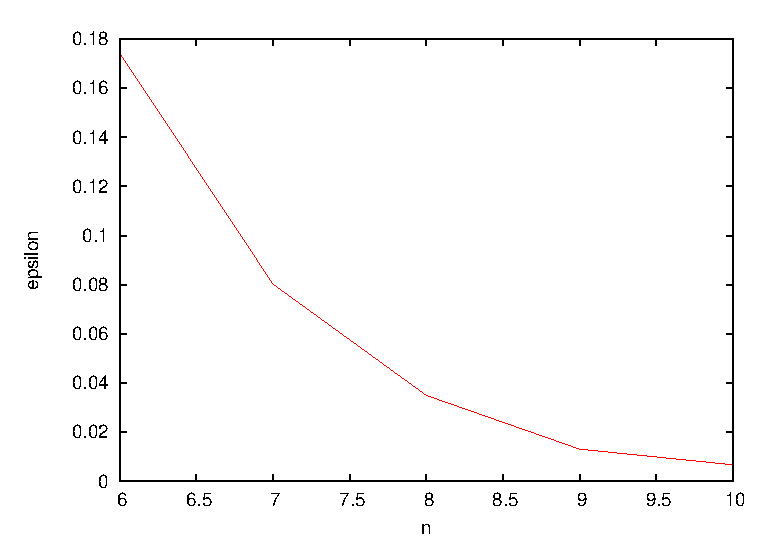
\includegraphics{converge_spatial}
    \caption{Plot showing the convergence of solutions based on changed in $\Delta x$. The computions are of $\epsilon_{\ell_1}$, $\epsilon_{\ell_2}$, and $\epsilon_{ell_\infty}$ with grid-size following $s(n) = 2^{n-1}+1$.}
    \label{fig:converge_spatial}
  \end{figure}

  The results from Figure \ref{fig:converge_spatial} show that the solutions converge as the grid size becomes refined.

%!% Also, check the results with a larger and smaller $\Delta t$ to see if they change.

%\subsubsection{$\Delta t$ Convergence}
%
%  A similar convergence analysis will also be performed for the temporal discritizations.
%  This is simply to confirm that the selection of $\Delta t$ is optimal for computation time and for accuracy.
%  The 
%
%  \begin{figure}
%    \centering
%    \begin{tabular}{c c}
%%    \includegraphics{converge_temporal_a.eps} &
%%    \includegraphics{converge_temporal_a.eps} \\
%    (a) & (b) \\
%%    \includegraphics{converge_temporal_a.eps} &
%%    \includegraphics{converge_temporal_a.eps} \\
%    (c) & (d)
%    \end{tabular}
%    \caption{A series of plots showing the convergece of solutions based on changes in $\Delta t$ using $eSoln = 10^n$ for (a) $n = -1$, (b) $n = -4$, (c) $n = -8$, and (d) $n = -12$.} 
%
%  \end{figure}
 
%\subsection{Table of Results}
%
%That list, compute time, "error", number of iterations of linear solver, and number of iterations for ALgorithm 1 for a series of $\epsilon_{sol}$.
%Do this table for a larger $\Delta t$ to see if the algorithm allows for a faster computation with the larger timesteps.
%
%Be extrodinaryly pedantic on everything here.
%Try for something like a paragraph for each item in the table; explain how it's computed, why we pick this measure, what we expect, and what it will say about the results....
%

\subsection{Results}
  Here the main comparison that analysis the effects of using Algorithm \ref{alg:iterateCM} with different $P$ values.
  Recall that the main observation is for $P = 1$, which corelates to the semi-implicit method. 
  Along with accuracy, the simulation time will be tracked.
  This is because it represents another metric for which the viability of the fully-implicit method can be verified.
  Theoretically there should be a decrease in the error with the fully-implicit method as the value for $P$ increases.
  Therefore, this needs to be weighted against the cost of computational intensity and the increase of the simulation time.

  %!% The fully-implicit method should have less iterations of the linear solver.
  
  The results of the method comparison can be seen in Table \ref{tab:tolerance_comparison}.

  %!% Have a table:
  %!%   tol. | avg iters | epsilon's | computer time| quantities of interest.... | (maybe avg iters of linear solver?)
  
  \begin{table}[h!tb]
    \centering
    %!% If I just list time and epsilons, maybe four gnuplots graph with the simulation time listed in the legend would be better.
    \begin{tabular}{|c|c|c|c|c|}
      \hline
      P & Simulation Time & $\epsilon_{\ell_1}$ & $\epsilon_{\ell_2}$ & $\epsilon_{\ell_\infty}$  \\
      \hline
      1& 60.05 & 0.0018 & - & - \\
      2& 97.72  & 0.0014 & - & - \\
      3& 117.46 & 0.0013 & - & - \\
      4& 126.44 & 0.0011& - & - \\
      \hline
      %!% OLD ROWS - Tol. 1 & Computation Time & $\epsilon_{sol}$ & Avg. Iter. 1 & Max Iter. 1 & Avg. Iter. 2 & Max Iter. 2 \\
    \end{tabular}
    \caption{Results from running simulation with different $P$ values. Note, $P = 1$ corresponds to the semi-implicit method.}
    \label{tab:tolerance_comparison}
  \end{table}
  
